\subsection{The DGMPM explicit discretization}
The continuum body $\Omega$ is discretized into a set of $N_p$ material points in an arbitrary Cartesian grid made of  $N_n$ nodes and $E$ non-overlapping cells of volume $\Omega^e $ (a two-dimensional example is depicted in figure \ref{fig:domain}).
% The boundary of the domain is again defined by the set of edges separating empty cells from those containing particles (see figure \ref{fig:domain} for a two-dimensional example).
\begin{figure}[ht]
  \centering
  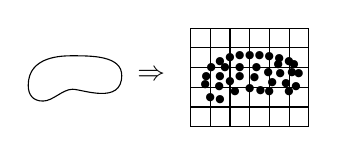
\begin{tikzpicture}[scale=0.25]
  % \draw[step=1.0,black,thin] (-3.,-1.) grid (3,4.);
  % \draw (-3,-1) -- (3,-1) -- (3,4) -- (-3,4) -- (-3,-1);
  \begin{scope}[scale=0.5]
    \draw (-3,0.6) .. controls +(1,0) and +(-1,0) .. (0,1.8)  
    .. controls +(1,0) and +(0,-3) .. (5,3.2) 
    .. controls +(0,2) and +(2,0)  .. (0,5.2) 
    .. controls +(-1,0) and +(0,3) .. (-4.5,2.2) 
    .. controls +(0,-1) and +(-1,0).. (-3,0.6) ;
    \begin{scope}  % pour limiter la portée du clip
      \clip (-3,0.6) .. controls +(1,0) and +(-1,0) .. (0,1.8) 
      .. controls +(1,0) and +(0,-3) .. (5,3.2)
      .. controls +(0,2) and +(2,0)  .. (0,5.2)
      .. controls +(-1,0) and +(0,3) .. (-4.5,2.2)
      .. controls +(0,-1) and +(-1,0).. (-3,0.6);
    \end{scope}
    %\node[below] at (0,1) {$\Omega$};
  \end{scope}
  \node at (4.,1.62) {$\Rightarrow$};
  \begin{scope}[shift={(9,0)}]
    \draw[step=1.0,black,thin] (-3.,-1.) grid (3,4.);
    % contour
    \node at (0,0.9) {\scriptsize$\bullet$}  ;
    \node at (2.5,1.65) {\scriptsize$\bullet$}  ; 
    \node at (0,2.6) {\scriptsize$\bullet$}  ;
    \node at (-2.25,1.1) {\scriptsize$\bullet$}  ; 
    \node at (-1.5,0.35) {\scriptsize$\bullet$}  ; 
    \node at (-2.,0.45) {\scriptsize$\bullet$} ;
    \node at (-2.2,1.5) {\scriptsize$\bullet$}  ; 
    \node at (-1.5,2.3) {\scriptsize$\bullet$} ; 
    \node at (2.35,1.) {\scriptsize$\bullet$}  ;
    \node at (2.25,2.15) {\scriptsize$\bullet$}  ;
    \node at (0.55,0.8) {\scriptsize$\bullet$}  ; 
    \node at (-0.5,2.6) {\scriptsize$\bullet$};
    \node at (0.5,2.59) {\scriptsize$\bullet$}  ;
    \node at (1.5,2.45) {\scriptsize$\bullet$}  ;
    \node at (1,0.75) {\scriptsize$\bullet$}; 
    \node at (2,0.75) {\scriptsize$\bullet$}  ;
    \node at (2,2.3) {\scriptsize$\bullet$}  ;
    \node at (1,2.55) {\scriptsize$\bullet$}  ;
    \node at (-1,2.5) {\scriptsize$\bullet$}  ; 
    \node at (-1.95,2.) {\scriptsize$\bullet$}  ;
    % interior
    \node at (-1.5,1.5) {\scriptsize$\bullet$}  ; 
    \node at (-1.25,2.) {\scriptsize$\bullet$}  ;
    \node at (-0.75,0.75) {\scriptsize$\bullet$}  ; 
    \node at (-1.55,1.){\scriptsize$\bullet$} ;
    \node at (-0.5,1.5) {\scriptsize$\bullet$}  ; 
    \node at (-0.5,2.) {\scriptsize$\bullet$}  ;
    \node at (0.25,1.45) {\scriptsize$\bullet$}  ;
    \node at (0.35,2.) {\scriptsize$\bullet$}  ;
    \node at (0.95,1.75) {\scriptsize$\bullet$}  ;
    \node at (1.15,1.2) {\scriptsize$\bullet$} ;
    \node at (1.45,2.15) {\scriptsize$\bullet$}  ; 
    \node at (1.55,1.65) {\scriptsize$\bullet$}  ;
    \node at (1.85,1.15) {\scriptsize$\bullet$}  ; 
    \node at (2.15,1.75) {\scriptsize$\bullet$}  ;
    \node at (-1.,1.25) {\scriptsize$\bullet$}  ;
    % \draw(3,0.5) -- (3.4,0.5) node [right]  {$\Omega_g$};
  \end{scope}
\end{tikzpicture}

%%% Local Variables:
%%% mode: latex
%%% TeX-master: "../presentation"
%%% End:

  \caption{Discretization of a two-dimensional solid domain using particles in an arbitrary grid.}
  \label{fig:domain}
\end{figure}
The particles are given a mass that enables the definition of the mass density in the grid by recourse to the Dirac delta function:
%In that grid, the reference mass density is described by means of the Dirac delta function and particle masses:
\begin{equation}
  \label{eq:mass_density_DGMPM}
  \rho_0\(\vect{X}\) =  \sum_{p=1}^{N_p} m_p \delta\(\vect{X}^p - \vect{X}\)
\end{equation}
In a similar manner to FEM \cite{Belytschko} and MPM \cite{Sulsky94}, the vector of conserved quantities is approximated on the mesh by:
\begin{equation}
  \label{eq:DGMPM_node2points}
  \Ucb(\vect{X},t) = \sum^{N_n}_{i=1} S_{i}(\vect{X})\Ucb^i(t) 
\end{equation}
with $\Ucb^i$ the vector of conserved quantities at node $i$, and $S_{i}(\vect{X})$ the (linear) shape function attached to it.
Note that particle and nodal quantities are respectively denoted with $p$ and $(i,j)$ subscripts or superscripts.

An approximate solution is sought by means of a weak form that results from multiplication of equation \eqref{eq:conservative_form} by a test function $\Wcb$ and integration over the grid.
According to the Discontinuous Galerkin approximation \cite{NeutronDG,Cockburn}, the test function belongs to a broken polynomial space \cite{DiPietro} in such a way that the weak form is written element-wise.
Thus, after integration by parts, one writes:
\begin{equation}
  \label{eq:DGMPM_weak_form}
  \int_{\Omega^e} \drond{\Ucb}{t} \Wcb \: d\Omega - \int_{\Omega^e} \Fcb_\alpha  \drond{\Wcb}{X_\alpha} \: d\Omega   + \int_{\partial \Omega^e} \Fcb_N  \Wcb \: dS = 0 \quad \forall \: \Wcb,e 
\end{equation}
where $\partial \Omega^e$ is the boundary of the $e$th element with outward normal vector $\vect{N}$.
Boundary integrals then involve interface fluxes $\Fcb_N=\Fcb\cdot \vect{N}$ enabling the propagation of information across cells, the computation of which is presented in section \ref{sec:riemann_solver}.

As for the original MPM \cite{Sulsky94,Sulsky95}, a particle-based quadrature can be used for volume integrals by considering specific fields:
\begin{equation}
  \label{eq:specific_quantities}
  \Ucb = \rho_0 \bar{\Ucb} \quad ; \quad \Fcb_\alpha = \rho_0 \bar{\Fcb}_\alpha
\end{equation}
Indeed, introduction of these fields and the definition of mass density \eqref{eq:mass_density_DGMPM} lead to the following total Lagrangian weak formulation:
\begin{equation} 
  \label{eq:DGMPM_discrete_weak}
  \sum_{p=1}^{N_p} m_p\[\drond{\bar{\Ucb}}{t}  \Wcb - \bar{\Fcb}_{\alpha} \drond{\Wcb}{X_\alpha} \]_{|\vect{X}=\vect{X}^p} + \int_{\partial \Omega^e} \Fcb_N  \Wcb \: dS = 0 \quad \forall \: \Wcb,e
\end{equation}

At last, the semi-discrete system is written by introducing the DGMPM approximation \eqref{eq:DGMPM_node2points} and considering the arbitrariness of the test function:
\begin{equation}
  \label{eq:DGMPM_semi_discrete}
  \sum_{p=1}^{N_p}\[ S_{ip} m_p S_{jp} \drond{\bar{\Ucb}^j}{t}  - \drond{S_{ip}}{X_\alpha} m_p S_{jp} \bar{\Fcb}^j_{\alpha} \] + \int_{\partial \Omega^e} S_i(\vect{X}) \Fcb_N  \: dS =  0  \quad \forall \: e
\end{equation}
or, in matrix form:
\begin{equation}
  \label{eq:DGMPM_semi_discrete_matrix}
  M_{ij} \drond{\bar{\Ucb}^j}{t} - K^\alpha_{ij} \bar{\Fcb}^j_{\alpha} + \vect{\hat{\Fc}}^i = \vect{0}  
\end{equation}
Note however that the particle-based quadrature may lead to a singular consistent mass matrix due to enventual reduced integrations \cite{Love}.
This issue can be circumvented by using the diagonally lumped mass matrix $M^L_i=\sum_j M_{ij}$.

The discrete system is derived by discretizing the time interval $\tau$ into $N_t$ subintervals and using the explicit forward Euler method:
\begin{equation}
  \label{eq:DGMPM_discrete}
  M^L_i \frac{\bar{\Ucb}^{i,n+1} - \bar{\Ucb}^{i,n}}{\Delta t^{n} } = K^\alpha_{ij} \bar{\Fcb}_{\alpha}^{j,n} - \vect{\hat{\Fc}}^{i,n}  
\end{equation}
where the superscripts $(\bullet)^{k,l}$ denote a field evaluated at node $k$ and time step $l$.
% \review{Alternatively, a \textit{second-order Runge-Kutta (RK2)} explicit time discretization may be employed, leading to the following two-stage discrete form:
% \begin{equation}
%   \label{eq:DGMPM_discrete_RK2}
%   \begin{aligned}
%     & M^L_i \frac{\bar{\Ucb}^{i,n+1/2} - \bar{\Ucb}^{i,n}}{\Delta t^{n} } = \frac{1}{2}\(K^\alpha_{ij} \bar{\Fcb}_{\alpha}^{j,n} - \vect{\hat{\Fc}}^{i,n}\)  \\
%     & M^L_i \frac{\bar{\Ucb}^{i,n+1} - \bar{\Ucb}^{i,n}}{\Delta t^{n} } = K^\alpha_{ij} \bar{\Fcb}_{\alpha}^{j,n+1/2} - \vect{\hat{\Fc}}^{i,n+1/2}
%   \end{aligned}
% \end{equation}
% \textit{
%   We chose here one existing two-stage second order Runge-Kutta method among others. See for instance \cite{Leveque} for a Total Variation Diminishing version of the RK2 time discretization. 
% }}

As for MPM, a discrete system is solved at nodes while the loading history is stored at material points.
Hence, a reconstruction of fields on the grid based on particle values is required as well as a projection of the updated solution from the grid to the material points.
The reconstruction procedure is similar to that used within the MPM and consists in ensuring the conservation of volume quantities:
\begin{equation}
  \label{eq:reconstruction}
  \bar{\Ucb}^{i,n} =  \frac{\sum_{p=1}^{N_p}S_{ip}m_p\bar{\Ucb}^{p,n}}{M_{i}^L }  \quad \text{for } i=1,...,N_n
\end{equation}
The back-mapping follows that proposed in the Particle-In-Cell method (PIC) \cite{PIC}, namely, a classical interpolation:
\begin{equation}
  \label{eq:back_mapping}
  \bar{\Ucb}^{p,n+1}=\sum_{i=1}^{N_n} S_{ip}\bar{\Ucb}^{i,n+1}
\end{equation}
Notice that the MPM is based on a different projection from nodes to particles that was introduced in the FLuid Implicit Particle method (FLIP) \cite{Mass_Flip}.
The FLIP mapping reduces the numerical diffusion resulting from the interpolation used in PIC at the cost of spurious oscillations.
The employment of the PIC projection rather than the FLIP one within the DGMPM is motivated by the willingness to avoid oscillations that can, for plastic materials, lead to a premature plastic flow due to overshoots in the stress values.
On the other hand, the diffusion inherent in PIC mapping is expected to be less significant with discontinuous shape functions due to the reduction of the domain of influence of nodes.

\subsection{Intercell fluxes}
%% Elastoplastic approximate Riemann solver for one-dimensional problems
%% Elastic Riemann solver + variational solver for multi-dimensional
\label{sec:riemann_solver}
% \begin{theorem}[Godunov \cite{Godunov_method}]
%   \label{th:Godunov}
%   Monotone linear numerical schemes can be at most first-order accurate.
% \end{theorem}

DG methods for hyperbolic problems are based on the requirement of ensuring monotonicity of the scheme for piecewise constant approximations \cite{Cockburn}. 
Such a numerical method is monotone for flux functions $\Fcb_N$ that are Lipschitz continuous, consistent and monotone, namely, they must be \textit{E-fluxes} \cite{Osher}.
One possibility, which is widely used and adopted here, is the \textit{Godunov flux function}. 

Let's consider the following Riemann problem that can be defined at the interface between two DGMPM cells having normal vector $\vect{N}$:
\begin{equation}
  \label{eq:RP_mesh}
  \begin{aligned}
    &\drond{\Ucb}{t} + \drond{\Fcb_N}{X_N} = \vect{0}  \\
    & \Ucb(X_N,0)= \left\lbrace 
      \begin{aligned}
        & \Ucb_{X_N^-} \text{ if } X_N < 0 \\
        & \Ucb_{X_N^{+}} \text{ if } X_N > 0
      \end{aligned}
        \right.
  \end{aligned}
\end{equation}
The intitial conditions $\Ucb_{X_N^-}$ and $\Ucb_{X_N^{+}}$ result from the average of nodal fields on each side of the interface, so that one Riemann problem is solved at each edge (see a two-dimensional example in figure \ref{fig:2D_edge}).

 
\begin{figure}[ht]
  \centering
  \begin{tikzpicture}[scale=0.5]
  \draw (10.,0.) -- (12.,6.) ; 
  \draw[fill=black] (9.85,0.1) circle (0.1) node [left] {$1$};	
  \draw[fill=black] (10.2,-0.0) circle (0.1) node [right] {$2$};	
  \draw[fill=black] (11.85,6.1) circle (0.1) node [left] {$4$};	
  \draw[fill=black] (12.2,6) circle (0.1) node [right] {$3$};	
  \draw[->,very thick] (11.,3.) -- (12,3 -1/3) node [right,below] {$X_N$}; 
  \node at (8,3.5) {$\vect{\Qc}_{L} = \frac{\vect{\Qc}_1 + \vect{\Qc}_4}{2}$}; \node at (14.5,3.5) {$\vect{\Qc}_{R} = \frac{\vect{\Qc}_2 + \vect{\Qc}_3}{2}$};
\end{tikzpicture}

  \caption{Duplication of nodes at an interface and building of initial conditions of the Riemann problem (2D).}
  \label{fig:2D_edge}
\end{figure}
The characteristic structure of the solution of problem \eqref{eq:RP_mesh} consists of waves emanating from the origin of the $(X_N,t)$ plane \cite{Courant}.
The wave pattern can be determined by the spectral analysis of the Jacobian matrix: $\Jbsf_\Uc = \drond{\Fcb_N}{\Ucb}$.
The eigenvalues $c_k$ and associated right eigenvectors $\Rcb^k$ ($k=1, ..., D$), $D$ being the dimension of the Jacobian, are respectively stored as diagonal entries and columns of matrices $\Cbsf$ and $\Rbsf$ which are defined as:
\begin{equation}
  \label{eq:eigen_matrices}
  \Jbsf_\Uc \Rbsf = \Rbsf \Cbsf
\end{equation}
% For flux vectors that are non-linear functions of $\Ucb$, as those involved for hyperelastic constitutive models, simple and shock waves may occur \cite{Wang} so that solving the problem drastically increases the computational cost.
For flux vectors that are non-linear functions of $\Ucb$, as those involved for hyperelastic constitutive models, solving problem \eqref{eq:RP_mesh} drastically increases the computational cost since this requires iterative procedures.
Nonetheless, linearized Riemann solvers \cite{Toro} can be constructed by approximating $\Jbsf_\Uc$ in the vicinity of $\Ucb_{X_N^-}$ and $\Ucb_{X_N^+}$ by a constant matrix $\underline{\Jbsf}(\Ucb_{X_N^-},\Ucb_{X_N^+})$.
The matrix $\underline{\Jbsf}$ must however ensure the hyperbolicity, namely $\underline{\Jbsf}$ has real eigenvalues and a complete set of independent eigenvectors \cite{Courant}, and satisfy the consistency condition \cite{Leveque}:
\begin{equation}
  \label{eq:consistency_Jacobian}
  \underline{\Jbsf}(\Ucb,\Ucb) = \Jbsf_\Ucb(\Ucb) 
\end{equation}
Both conditions can be satisfied by assuming that the negative (\textit{resp. positive}) eigenvalues and the associated right eigenvectors of $\Jbsf_\Ucb$, which correspond to left-going (\textit{resp. right-going}) waves, depend only on  $\Ucb_{X_N^-}$ (\textit{resp. on $\Ucb_{X_N^+}$}).
Then, defining the matrices:
\begin{align*}
  &\underline{\Cbsf}=\matrice{c_1(\Ucb_{X_N^-}) & & & & & \\ & \cdots & & && \\ & &c_I(\Ucb_{X_N^-}) & & &\\ & & &c_{I+1}(\Ucb_{X_N^+})& & \\ & & & &\cdots &\\ &&&&&c_D(\Ucb_{X_N^+})} \\
  &\underline{\Rbsf} = \matrice{\Rcb^1(\Ucb_{X_N^-}),\:  ...\:  ,\: \Rcb^I(\Ucb_{X_N^-}),\: \Rcb^{I+1}(\Ucb_{X_N^+}),\:...\: ,\: \Rcb^D(\Ucb_{X_N^+})} 
\end{align*}
in which $c_1<\cdots <c_I<c_{I+1}<\cdots < c_D$, the following approximation fulfills the requirements provided that $\Jcb_\Uc$ ensures the hyperbolicity:
\begin{equation}
  \label{eq:3}
  \underline{\Jbsf} = \underline{\Rbsf} \: \underline{\Cbsf} \: \underline{\Rbsf}^{-1}
\end{equation}

Though approximate-flux Riemann solvers, which extract information for flux functions, have been applied to hyper solids (see Osher's solver in \cite{Haider_FVM,Lee_FVM} or the HLLC solver in \cite{Ortega_HLLD}), the approximate-state Riemann solver is considered here.
The procedure then consists in computing the stationary solution of the linearized Riemann problem as \cite{Toro}:
\begin{equation}
  \label{eq:stationary_solution}
  \Ucb^* = \Ucb_{X_N^-} + \sum_{\underset{c_k < 0}{k=1}}^D \delta_k\Rcb^k = \Ucb_{X_N^+} - \sum_{\underset{c_k > 0}{k=1}}^D \delta_k\Rcb^k
\end{equation}
where the $\delta_k$ are wave strength coefficients related to the $k$th wave of the characteristic structure.
These coefficients can be computed by rearranging equation \eqref{eq:stationary_solution} as:
\begin{equation}
  \label{eq:delta_U}
  \Ucb_{X_N^+} - \Ucb_{X_N^-} = \sum_{k=1}^D \delta_k\Rcb^k
\end{equation}
so as to compute the stationary solution.
Once $\Ucb^*$ is known, the intercell flux is computed as $\Fcb_N\(\Ucb^*\)$ according to Godunov's method \cite{Godunov_method}.
Since the vector of conserved quantities $\Ucb$ contains the deformation gradient and the linear momentum while the flux is composed of stress and velocity, the integration of constitutive equations, which may be costly, is required. 
This can however be avoided by formulating the Riemann problem based on the quasi-linear form \eqref{eq:quasi-linear} involving velocity and stress, thus allowing the direct computation of intercell fluxes through the auxiliary vector $\Qcb$.
This approch then requires that stress as well as velocity and strain are projected from the material points to the nodes by means of the reconstruction \eqref{eq:reconstruction}.

% \begin{remark}
% Hyperbolic systems having zero eigenvalues lead to stationary waves, propagating at zero celerity, across which the solution of the Riemann problem may have discontinuities.
%   In that case, the associated Godunov flux is also discontinuous so that one stationary state must be considered on both sides of the characteristic.
%   This approach leads to the computation of two fluxes, each contributing to one cell only. 
% \end{remark}

\begin{remark}
  The approximate-state Riemann solver described above allows to account for the transverse propagation of waves by adding correction terms on the intercell fluxes similarly similarly to the Corner Transport Upwind method (CTU) \cite{Colella_CTU}.
  The use of the CTU within the DGMPM, presented in \cite{DGMPM}, enables the improvement of the stability properties of the scheme for problems involving Poisson's effect \cite{Thesis}.
\end{remark}


As seen in section \ref{sec:continuum_problem}, the Jacobian matrix of the system involves the fourth-order tangent modulus tensor.
However, this tensor is responsible for a more complex characteristic structure when plastic flow occurs since one has to take into account both elastic and plastic waves in that case \cite{Wang}.
For small strain problems, the corresponding characteristic structure is known in particular cases so that dedicated Riemann solvers have been developed for one-dimensional media \cite{Thomas_EP} or for combined longitudinal and torsional stress loadings \cite{Lin_et_Ballman}.
Given the complexity introduced by finite deformations, such solvers cannot be considered.
As a result, a purely reversible evolution is commonly considered for the computation of intercell fluxes, followed by the integration of the plastic flow by using a return mapping algorithm in finite volume simulations (see \cite{FRRSE,Maire_elastoplast} for hypoelastic-plastic materials and \cite{Lee_FVM} for hyperelastic-plastic ones).
A similar approach is adopted here in such a way that the DGMPM scheme consists in a predictor-corrector procedure, the integration of plastic flow being carried out through variational constitutive updates.
This is the object of the next section.



%%% Local Variables:
%%% mode: latex
%%% TeX-master: "manuscript"
%%% End:
